\documentclass[xcolor={dvipsnames}]{beamer}
\usepackage[utf8]{inputenc}


\usepackage{tikz}
\usetikzlibrary{calc}
\usetikzlibrary{arrows.meta}
\usetikzlibrary{backgrounds,matrix,fadings,calc,positioning,decorations.pathreplacing,arrows.meta,shapes,shapes.multipart}
\usepackage{standalone} % Necessary to skip headers of {standalone} documents
\usepackage{tikzscale} % To use \includegraphics with TikZ code
\usetikzlibrary{backgrounds,fit,positioning}

\usepackage{graphicx} % Include the package for graphics
% Nummerrierung von Abbilungen und Tabelle fortlaufend
\usepackage{chngcntr}

% Paket für Tabellen im Corporate Design der Universität Konstanz
\usepackage{tabu}
\usepackage{array,booktabs,ragged2e}
\usepackage{pgfplots}
\usepackage[normalem]{ulem}



%%%%%%%%%%%%%%%%%%%%%%%%%%%%%%%%%%%%%%%%%%%%%%%%%%%%%%%%%
% Tabellenzusatzpezifikationen                          %
%%%%%%%%%%%%%%%%%%%%%%%%%%%%%%%%%%%%%%%%%%%%%%%%%%%%%%%%%

\newcolumntype{L}[1]{>{\raggedright\arraybackslash}p{#1}}
\newcolumntype{C}[1]{>{\centering\arraybackslash}p{#1}}
\newcolumntype{R}[1]{>{\raggedleft\arraybackslash}p{#1}}

\usetheme{Madrid}
\usecolortheme{default}
\setbeamertemplate{enumerate items}[default]
\definecolor{uniBlau}{RGB}{59,199,235}
\setbeamercolor*{structure}{bg=white,fg=uniBlau}

% \setbeamercolor*{palette primary}{use=structure,fg=white,bg=structure.fg}
% \setbeamercolor*{palette secondary}{use=structure,fg=white,bg=structure.fg!75}
% \setbeamercolor*{palette tertiary}{use=structure,fg=white,bg=structure.fg!50!black}
% \setbeamercolor*{palette quaternary}{fg=white,bg=black}

% \setbeamercolor{section in toc}{fg=black,bg=white}
% \setbeamercolor{alerted text}{use=structure,fg=structure.fg!50!black!80!black}
% \setbeamercolor{frametitle}{bg=black,fg=white}

% \setbeamercolor{titlelike}{parent=palette primary,fg=structure.fg!50!black}
% \setbeamercolor{frametitle}{bg=gray!10!white,fg=black}

% \setbeamercolor*{titlelike}{parent=palette primary}

% \setbeamercolor{block title example}{bg=black,fg=white}

% \usepackage{times,url}

% \setbeamertemplate{footline}[frame number]
% \setbeamertemplate{footline}[frame number]{}

%\setbeamertemplate{footline}{}

%\setbeamertemplate{footline}
%{
%  \leavevmode%
%  \hbox{%
%  \begin{beamercolorbox}[wd=.333333\paperwidth,ht=2.25ex,dp=1ex,center]{author in head/foot}%
%    \usebeamerfont{author in head/foot}\insertsection
%  \end{beamercolorbox}%
%  \begin{beamercolorbox}[wd=.333333\paperwidth,ht=2.25ex,dp=1ex,center]{title in head/foot}%
%    \usebeamerfont{title in head/foot}\insertsubsection
%  \end{beamercolorbox}%
%  \begin{beamercolorbox}[wd=.333333\paperwidth,ht=2.25ex,dp=1ex,right]{date in head/foot}%
%    \usebeamerfont{date in head/foot}\insertshortdate{}\hspace*{2em}
%    \insertframenumber{} / \inserttotalframenumber\hspace*{2ex} 
%  \end{beamercolorbox}}%
%  \vskip0pt%
%}

%------------------------------------------------------------
%This block of code defines the information to appear in the
%Title page
\title[CCH in Neo4j] %optional
{Query Processing on Dynamic Networks with Customizable Contraction Hierarchies on Neo4j}

%\subtitle{A short story}

\author[Marius Hahn] % (optional)
{Marius Hahn}

\institute[CIS] % (optional)
{
  Grouf of Database and Information Systems \\
  Department of Computer and Information Science \\
  Faculty of Sciences \\
  Universität Konstanz
}

\date[$\text{14}^{\text{th}}$ December 2023] % (optional)
{Master Colloquium, $\text{14}^{\text{th}}$ December 2023}

% 右下角使用logo的方式
% \logo{\includegraphics[height=1cm]{overleaf-logo}} 

%End of title page configuration block
%------------------------------------------------------------



%------------------------------------------------------------
%The next block of commands puts the table of contents at the 
%beginning of each section and highlights the current section:

\AtBeginSection[]
{
  \begin{frame}
    \frametitle{Table of Contents}
    \tableofcontents[currentsection]
  \end{frame}
}
%------------------------------------------------------------


\begin{document}

%The next statement creates the title page.
\frame{\titlepage}


%---------------------------------------------------------
%This block of code is for the table of contents after
%the title page
\begin{frame}
\frametitle{Table of Contents}
\tableofcontents
\end{frame}
%---------------------------------------------------------

\section{Introduction}
\begin{frame}
    \frametitle{Motivation and Context}
    \begin{itemize}
        \item Graph Databases $\Rrightarrow$ External memory
        \item Accelerate Shortest Path Queries in Databases 
        \item Why Customizable Contraction Hierarchies? 
        \begin{itemize}
            \item fast for main memory applications
            \item reasonable preprocessing time
            \item It is updatable
        \end{itemize}
        \item Test Data $\Rrightarrow$ Road Networks
    \end{itemize}

\end{frame}
\begin{frame}
    \frametitle{Obstacles}

    \begin{columns}
        \column{0.7\textwidth}

        \textbf{Property Graph:}
        \vfill
        \centering
        \includegraphics[width=0.8\linewidth]{assets/tikz/obstaclePropertyGraph.tex}
        \column{0.3\textwidth}
        \visible<2->{\textbf{File:}\\
        \vfill
        \centering
        \includegraphics[width=0.8\linewidth]{assets/tikz/file.tex}}
    \end{columns}
    \vfill
    \begin{itemize}
        \item<3-> transformation to data structure with a single dimension
        \item<4-> Databases use HDDs $\Rrightarrow$ slow random access
    \end{itemize}

    
\end{frame}

\section{Dijkstra}
\begin{frame}
    \frametitle{Dijkstra}
    Let's go from $v_2$ to $v_3$
    \vfill
    \begin{columns}
    \column{0.5\textwidth}
    \centering
    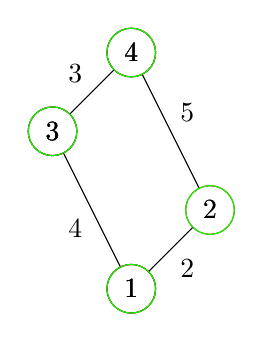
\begin{tikzpicture}[node distance={15mm}, main/.style = {draw, circle}]
        
        \onslide<1-2>{\node[main] (x3) at (0, 2) {$3$};}
        \onslide<3-4>{\node[main, draw=red] (x3) at (0, 2) {$3$};}
        \onslide<5->{\node[main, draw=green] (x3) at (0, 2) {$3$};}
        \onslide<1>{\node[main] (x4) at (1, 3) {$4$};}
        \onslide<2-3>{\node[main, draw=red] (x4) at (1, 3) {$4$};}
        \onslide<4->{\node[main, draw=green] (x4) at (1, 3) {$4$};}
        \onslide<1>{\node[main, draw=red] (x2) at (2, 1) {$2$};}
        \onslide<2->{\node[main, draw=green] (x2) at (2, 1) {$  2$};}
        \onslide<1>{\node[main] (x1) at (1, 0) {$1$};}
        \onslide<2>{\node[main, draw=red] (x1) at (1, 0) {$1$};}
        \onslide<3->{\node[main, draw=green] (x1) at (1, 0) {$1$};}
        
        \draw (x1) -- node[below right] {$2$}(x2);
        \draw (x1) -- node[below left] {$4$} (x3);
        \draw (x2) -- node[above right] {$5$} (x4);
        \draw (x3) -- node[above left] {$3$} (x4);

    \end{tikzpicture}
    \column{0.5\textwidth}
    \centering
    \begin{tabular}{c | c | c}
        \textbf{id} & \textbf{dist} & \textbf{settled}\\
        \hline 
        2 & 0  & \onslide<1>{false} \onslide<2->{true} \\ 
        \hline \pause
        1 & 2 & \onslide<2>{false} \onslide<3->{true}\\ 
        \hline
        4 &  5 & \onslide<2-3>{false} \onslide<4->{true} \\
        \hline \pause
        3 & 6 & \onslide<3-4>{false} \onslide<5->{true}\\ 
    \end{tabular}
\end{columns}
          
    

\end{frame}

\section{Contraction Hierarchies}
\begin{frame}
    \frametitle{Contraction Hierarchies Example}

    \visible<5->{Let's go from $v_2$ to $v_3$}
    \vfill
    \centering
    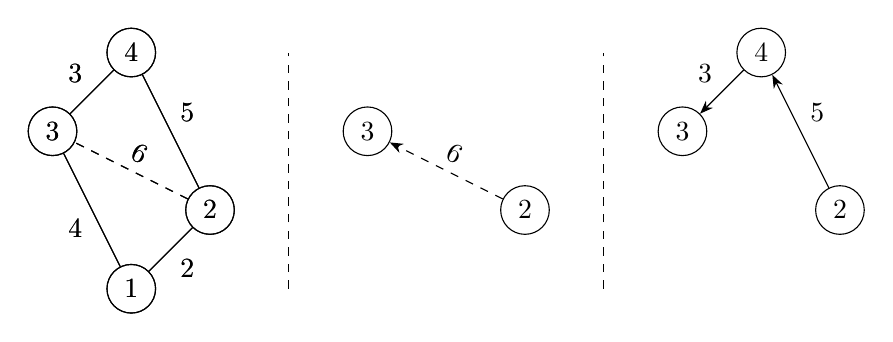
\begin{tikzpicture}[node distance={15mm}, main/.style = {draw, circle}]
        \visible<1-4>{\node[main] (x4) at (1, 3) {$4$};}
        \visible<1-3>{\node[main] (x3) at (0, 2) {$3$};}
        \visible<1-2>{\node[main] (x2) at (2, 1) {$2$};}
        \visible<1>{\node[main] (x1) at (1, 0) {$1$};}
        \visible<5->{\node[main] (x4) at (1, 3) {$4$};}
        \visible<5->{\node[main] (x3) at (0, 2) {$3$};}
        \visible<5->{\node[main] (x2) at (2, 1) {$2$};}
        \visible<5->{\node[main] (x1) at (1, 0) {$1$};}
        
        \visible<1>{\draw (x1) -- node[below right] {$2$}(x2);}
        \visible<1>{\draw (x1) -- node[below left] {$4$} (x3);}
        \visible<1-2>{\draw (x2) -- node[above right] {$5$} (x4);}
        \visible<1-3>{\draw (x3) -- node[above left] {$3$} (x4);}
        \visible<2>{\draw[dashed] (x2) -- node[above, sloped] {$6$}  (x3);}
        \visible<5->{\draw (x1) -- node[below right] {$2$}(x2);}
        \visible<5->{\draw (x1) -- node[below left] {$4$} (x3);}
        \visible<5->{\draw (x2) -- node[above right] {$5$} (x4);}
        \visible<5->{\draw (x3) -- node[above left] {$3$} (x4);}
        \visible<5->{\draw[dashed] (x2) -- node[above, sloped] {$6$}  (x3);}
    
        \visible<6->{\draw[dashed]  (3,0) -- (3,3);}
    
    
        \visible<7->{\node[main] (x31) at (4, 2) {$3$};}
        \visible<6->{\node[main] (x21) at (6, 1) {$2$};}
        \visible<7->{\draw[ -Stealth, dashed] (x21) to node[above, sloped] {$6$}  (x31);}
    
        \visible<6->{\draw[dashed]  (7,0) -- (7,3);}
    
        \visible<8->{\node[main] (x32) at (8, 2) {$3$};}
        \visible<7->{\node[main] (x42) at (9, 3) {$4$};}
        \visible<6->{\node[main] (x22) at (10, 1) {$2$};}
    
        \visible<7->{\draw[-Stealth,] (x22) to node[above right] {$5$} (x42);}
        \visible<8->{\draw[-Stealth] (x42) to node[above left] {$3$} (x32);}
    
\end{tikzpicture}

\end{frame}
\begin{frame}
    \frametitle{Customizable Contraction Hierarchies}
    \begin{itemize}
        \item CH insert shortcut if shortest path property is violated
        \item CCH insert shortcut if there is no direct connection
    \end{itemize}
    \vfill
    \centering
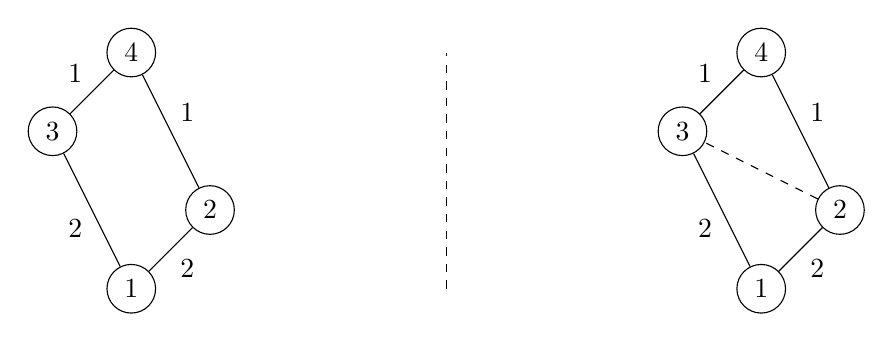
\begin{tikzpicture}[node distance={15mm}, main/.style = {draw, circle}]

    \node[main] (x3) at (0, 2) {$3$};
    \node[main] (x4) at (1, 3) {$4$};
    \node[main] (x2) at (2, 1) {$2$};
    \node[main] (x1) at (1, 0) {$1$};
    
    \draw (x1) -- node[below right] {$2$}(x2);
    \draw (x1) -- node[below left] {$2$} (x3);
    \draw (x2) -- node[above right] {$1$} (x4);
    \draw (x3) -- node[above left] {$1$} (x4);

    \draw[dashed]  (5,0) -- (5,3);

    \node[main] (x31) at (8, 2) {$3$};
    \node[main] (x41) at (9, 3) {$4$};
    \node[main] (x21) at (10, 1) {$2$};
    \node[main] (x11) at (9, 0) {$1$};
    
    \draw (x11) -- node[below right] {$2$}(x21);
    \draw (x11) -- node[below left] {$2$} (x31);
    \draw (x21) -- node[above right] {$1$} (x41);
    \draw (x31) -- node[above left] {$1$} (x41);
    \draw[dashed] (x21) -- node[above, sloped] {}  (x31);

    
\end{tikzpicture}
\end{frame}
\begin{frame}
    \frametitle{CCH Weights | Lower Triangles}
    \includegraphics[width=\linewidth]{assets/tikz/lowerTriangle.tex}
    \visible<3>{\begin{alertblock}{} \centering
        Bottom up for every arc! Also original arcs
    \end{alertblock}}
\end{frame}
\begin{frame}
    \frametitle{CCH Update | Upper Triangle}
    \begin{itemize}
        \item Check if edge(y,z) could rely in edge(x,y)
        \item If yes $\Rrightarrow$ redo lower triangles for e(y,z)
    \end{itemize}

    \includegraphics[width=\linewidth]{assets/tikz/upperTriangle.tex}

\end{frame}
\begin{frame}
    \frametitle{CCH Update | Intermediate Triangle}
    \begin{itemize}
        \item Check if edge(y,z) could rely in edge(x,y)
        \item If yes $\Rrightarrow$ redo lower triangles for e(y,z)
    \end{itemize}

    \includegraphics[width=\linewidth]{assets/tikz/intermediateTriangle.tex}
\end{frame}

\section{Vertex Order}
\begin{frame}
    \frametitle{Important vertex not contraced Last}
    \begin{itemize}
        \item Contracted Using Edge Difference
        \item Go from v(1) to v(3)
        \item Forward and Backward search are deeper that the should be
        \item Switch contraction order of v(4) and v(5)
    \end{itemize}
    \vfill
    \centering
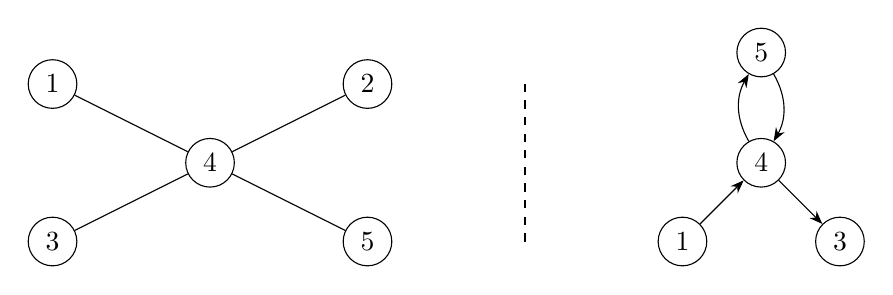
\begin{tikzpicture}[node distance={15mm}, main/.style = {draw, circle}]
    \node[main] (x1) at (0, 2) {$1$}; 
    \node[main] (x3) at (0, 0) {$3$};
    
    \node[main] (x4) at (2, 1) {$4$}; 
    
    \node[main] (x2) at (4, 2) {$2$}; 
    \node[main] (x5) at (4, 0) {$5$}; 
    
    \draw (x1) -- (x4);
    \draw (x2) -- (x4);
    \draw (x3) -- (x4);
    \draw (x5) -- (x4);

    \draw[dashed]  (6,0) -- (6,2);


    \node[main] (x1) at (8, 0) {$1$};
    \node[main] (x3) at (10, 0) {$3$};
    \node[main] (x4) at (9, 1) {$4$};
    \node[main] (x5) at (9, 2.4) {$5$};

    \draw[ -Stealth] (x1) -- (x4);
    \draw[ -Stealth] (x4) -- (x3);

    \draw[ -Stealth, out=120, in=-120] (x4) to (x5);
    \draw[ -Stealth, out=-60, in=60] (x5) to (x4);

\end{tikzpicture} 
\end{frame}
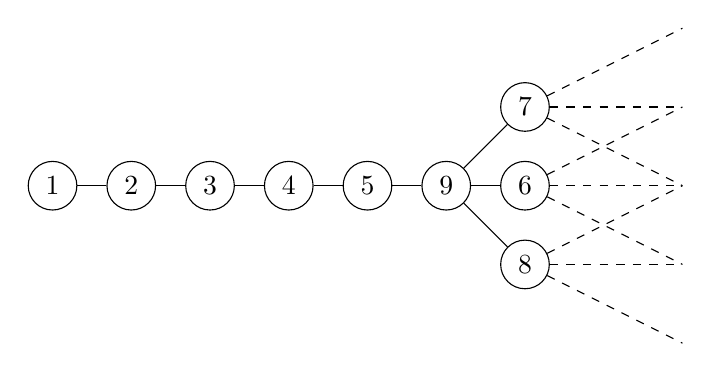
\begin{tikzpicture}[node distance={15mm}, main/.style = {draw, circle}]

    \node[main] (x1) at (0, 0) {$1$};
    \node[main] (x2) at (1, 0) {$2$};
    \node[main] (x3) at (2, 0) {$3$};
    \node[main] (x4) at (3, 0) {$4$};
    \node[main] (x5) at (4, 0) {$5$};
    \node[main] (x9) at (5, 0) {$9$};
    
    \node[main] (x7) at (6, 1) {$7$};
    \node[main] (x8) at (6, -1) {$8$};
    \node[main] (x6) at (6, 0) {$6$};
    
    
    \draw (x1) -- (x2);
    \draw (x2) -- (x3);
    \draw (x3) -- (x4);
    \draw (x4) -- (x5);
    \draw (x5) -- (x9);
    
    \draw (x6) -- (x9);
    \draw (x9) -- (x7);
    \draw (x9) -- (x8);
    
    \draw [dashed] (x7) -- (8, 2);
    \draw [dashed] (x7) -- (8, 1);
    \draw [dashed] (x7) -- (8, 0);
    
    \draw [dashed] (x8) -- (8, 0);
    \draw [dashed] (x8) -- (8, -2);
    \draw [dashed] (x8) -- (8, -1);
    
    \draw [dashed] (x6) -- (8, 1);
    \draw [dashed] (x6) -- (8, 0);
    \draw [dashed] (x6) -- (8, -1);
    
\end{tikzpicture} 
    
\begin{frame}
    \frametitle{Importance Calculation}

    \begin{itemize}
        \item add a level $l(v) = 0$ to each node 
        \item if contracting v: $l(v) = max\{l(v)+1, l(w)\} \forall w \epsilon N(v)$
        \item $A(v)$ set of added arcs
        \item $D(v)$ set of deleted arcs
        \item $h(a)$ hops an arc represents if unpacked
    \end{itemize}

    \begin{equation*}
        \label{eq:importance}
        i(v) = l(v) + \frac{|A(v)|}{|D(v)|} + \frac{\sum_{a \epsilon A(v)} h(a)}{\sum_{a \epsilon D(v)} h(a)} 
    \end{equation*}
    
    \begin{alertblock}{Important theorem}
        more shortcuts inserted but improves query time!
    \end{alertblock}
\end{frame}

\section{External Memory}
\begin{frame}
    \frametitle{Persistance Objectives}
    \centering
    \includegraphics[width=0.7\linewidth]{assets/tikz/propertyGraph.tex}
    \begin{itemize}
        \item keep only necessary data
        \begin{itemize}
            \item \textcolor{red}{rank} $\rightarrow$ to do the mapping to the input graph
            \item arc \textcolor{red}{weight}
        \end{itemize}
        \item Store edges that are likely to be request together spacial close
        \item Use as few space as possible $\rightarrow$ the less you write the less you read
    \end{itemize}
\end{frame}
\begin{frame}
    \frametitle{Magnetic Disks}
    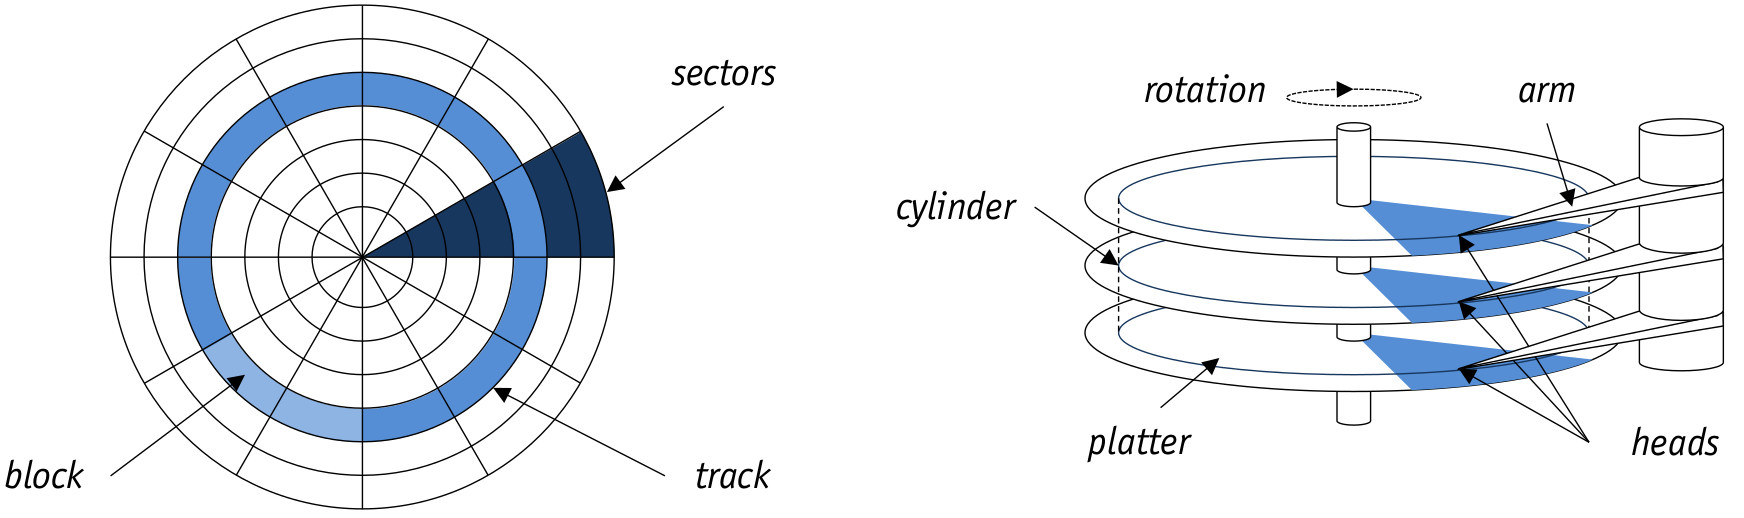
\includegraphics[width=1\linewidth]{assets/images/magneticDisks.png}
    \begin{itemize}
        \item Data is arranged in concentric rings (tracks) on platters 
        \item Tracks are divided into arc-shaped sectors
    \end{itemize}
    \begin{alertblock}{One by One}
        Data is read from and written to disk one \textbf{block} at a time
        \end{alertblock}
\end{frame}
\begin{frame}
    \frametitle{Transformation to a Table}
    \begin{itemize}
        \item Depth-First-Search starting at highest rank
        \item retrieve only arcs. vertices will be reconstructed form arcs
        \item remember middle node
    \end{itemize}
    \centering
    \includegraphics[width=0.7\linewidth]{assets/tikz/propertyGraphWithTable.tex}

\end{frame}
\begin{tikzpicture}[node distance={15mm}, main/.style = {draw, circle}]
    
    \draw (-7,6) rectangle (-1,7);
    \draw (-5.5,6) -- (-5.5,7);
    \draw (-4,6) -- (-4,7);
    \draw (-2.5,6) -- (-2.5,7);
    \node at (-6.25, 6.5) {from};
    \node at (-4.75, 6.5) {to};
    \node at (-3.25, 6.5) {middle};
    \node at (-1.75, 6.5) {weight};

    \draw [decorate,decoration = {brace, amplitude=5pt}] (-7,7.1) --  (-5.5,7.1);
    \draw [decorate,decoration = {brace, amplitude=5pt}] (-5.5,7.1) --  (-4,7.1);
    \draw [decorate,decoration = {brace, amplitude=5pt}] (-4,7.1) --  (-2.5,7.1);
    \draw [decorate,decoration = {brace, amplitude=5pt}] (-2.5,7.1) --  (-1,7.1);
    \node[ align=center] at (-6.25, 7.8) {32 bit  \\ integer};
    \node[ align=center] at (-4.75, 7.8) {32 bit  \\ integer};
    \node[ align=center] at (-3.25, 7.8) {32 bit  \\ integer};
    \node[ align=center] at (-1.75, 7.8) {32b bit \\ integer};

    \draw [decorate,decoration = {brace, amplitude=5pt}] (-1,5.9) --  (-7, 5.9);
    \node at (-4, 5.5) {16 byte disk arc};

    \draw[dashed, -Stealth] (-1,7) -- (0, 6.7);
    \draw[dashed, -Stealth] (-1,6) -- (0, 6.3);
    
    
    \draw (0,7) -- (4,7);
    \draw[dashed] (0,6) -- (4,6);
    \draw[dashed] (0,5) -- (4,5);
    \node at (4.5,5) {0};
    \node at (4.5,1) {1};
    \draw (0,3) -- (5,3); 
    \draw[dashed] (0,2) -- (4,2);
    \draw[dashed] (0,1) -- (4,1);
    \draw[out=60, in=-120] (0,0) to (4, 0);
    \draw (0,0) -- (0,7); 
    \draw (4,0) -- (4,7); 
    \node at (2, 6.5) {disk arc};
    \node at (2, 5.5) {disk arc};
    \node[rotate=90, font=\Large] at (2, 4) {. . . . .};
    
    \node[rotate=-90] at (5.85, 5) {disk block};
    \draw [decorate,decoration = {brace, amplitude=10pt}] (5.2,7) --  (5.2,3);
\end{tikzpicture}
\begin{frame}
    \frametitle{CCH Disk Search (upwards graph example)}

    \begin{enumerate}
        \item lazy load vertices $\Rrightarrow$ only start node is loaded without arcs 
        \item<2-> settle vertex (right before expanding it) 
        \begin{itemize}
            \item<3-> VertexManager requests arc of v(x) from buffer
            \item<4-> Buffer requests arcs from disk if not cached yet
            \item<6-> Buffer returns arcs
            \item<7-> VertexManager attaches arcs to v(x)
        \end{itemize}
    \end{enumerate}
    \vfill
    \includegraphics[width=\linewidth]{assets/tikz/lazyLoadVertex.tex}
    

\end{frame}
\begin{frame}
    \frametitle{Circular Buffer}
    \includegraphics[width=\textwidth]{assets/tikz/CircularBuffer.tex}
    \onslide<7>{    
    \begin{itemize}
        \item Retrieve Arcs $\Rrightarrow$ iterate backwards from position until start vertex differs
        \item If arc is doesn't start with requested rank $\Rrightarrow$ remove position and refetch
    \end{itemize}}

\end{frame}

\section{Experiments}
\begin{frame}
    \frametitle{General Results}
    \centering
        \includegraphics[width=0.95\linewidth]{assets/tables/experimentKeyTable.tex}
\end{frame}


\begin{frame}
    \frametitle{Dijkstra vs. CCH | Query Time}

    \centering
    \includegraphics[height=0.65\linewidth]{assets/plots/dijkstra-vs-cch-query-speed.tex}

\end{frame}
\begin{frame}
    \frametitle{Expanded Vertices}
    \centering
    \includegraphics[height=0.43\linewidth]{assets/plots/dijkstra-vs-cch-expanded-vertices.tex}   
\end{frame}
\begin{frame}
    \frametitle{Buffer 640 kB}
    \centering
    \includegraphics[height=0.65\linewidth]{assets/plots/io-comparison.tex}

\end{frame}
\begin{frame}
    \frametitle{Buffer 20\% Arc Count}

    \includegraphics[height=0.43\linewidth]{assets/plots/coloradoBufferComp.tex}

\end{frame}

\section{Conclusion}
\begin{frame}
    \frametitle{Conclusion}
    
    \begin{itemize}
        \item We can accelerate Graph Databases with CCH
        \item The major problem is to flatten the graph
        \item Try it with a Relational Database
    \end{itemize}

\end{frame}

\end{document}